\chapter{Überblick -- Multi-Cloud-Anwendungs-Brokering}
\label{cha:broker}

% Vorteile
% Neue Märkte in anderen Regionen der Welt
% Schnelles Ausrollen neuer Apps
% DevOps geeignet
% Risikoreduzierung
% Reduzierung von (gleichzeitig) Investitionsausgaben und Betriebskosten
% Bestehende Cloud-Deployments mit verwalten-

Um eine Anwendung automatisiert auf verschiedene Clouds zu verteilen, ist ein Broker-Mechanismus nötig. Dieser sollte nach verschiedenen, festzulegenden Kriterien vorgehen. Konkret erfüllt ein Broker in der Regel folgende Aufgaben \cite{gartner:2017:cloud-market-multicloud-trend}:

\begin{enumerate}
	\item Bereitstellen der Ressourcen für eine Applikation; starten einer virtuellen Maschine oder Reservierung von Speicherplatz
	\item Starten der Anwendung auf den vorher reservierten Ressourcen
	\item Verteilen eingehender Anfragen auf gestartete Anwendungs-Instanzen
	\item Management der Ressourcen
\end{enumerate}

\noindent
Zusätzlich sollte der Multi-Cloud-Broker Policys und SLAs auswerten und umsetzen können. Denkbar ist das automatische Re-provisionieren anhand von 

\begin{enumerate}
	\item Lastspitzen oder Ausfällen von Hardware und Netzwerkressourcen 
	%	(Monitoring)
	\item Geänderten Umfeldparametern wie der Gesetzgebung, Preisen oder AGBs
	\item Nutzeränderungen
	\item Vorherigen Broker-Aktionen
\end{enumerate}

\noindent
In einer Community-Cloud könnten Cloud-Provider selbst einen Mechanismus zum Brokering oder zumindest offene APIs bereitstellen. Der Broker wäre also Teil der Cloud. Möglich sind entweder ein zentraler Broker, der direkt auf Cloud-Interna zugreift, oder aber ein Peer-to-Peer-Verbund.\todo{Grafik Architekturübersicht}

Für Multi-Clouds kommen diese Lösungen nicht infrage: Sie bestehen aus mehreren unabhängigen, meist privaten, Cloud-Providern. Aufgrund gegenläufiger Geschäftsinteressen sind diese nicht an einer Föderation mit anderen Anbietern interessiert. Sie werden also weder Interna ihrer Cloud-Plattform anpassen, noch einheitliche APIs bereitstellen.

Stattdessen muss der Broker in einer Multi-Cloud-Umgebung extern bereitgestellt werden. In diesem Fall kann er, entweder als eigenständiger Service in Form einer \emph{Cloud-Management-Plattform} angelegt sein, oder von der verteilten Anwendung selbst implementiert werden. Selbst entwickelte CMPs oder integrierte Broker setzen oft auf Multi-Cloud-Bibliotheken wie \emph{Apache libcloud}. \autoref{sec:bibliotheken} bietet hierzu eine Übersicht aktueller Open-Source-Projekte. 

Folgende weitere Aspekte sollen bei der Betrachtung der CMPs berücksichtigt werden:

\begin{description}
	
	\item[Zielgruppe] 	\emph{Entwickler und Administratoren}: Im Rahmen von DevOps stellen sie verschiedene Ausführungsumgebungen für Entwicklung, Test und Produktion bereit. Dabei nutzen sie die Self-Service-Funktionen der CMPs.
	
						\emph{Management}: Die Auslastungs- und Kostenübersicht ermöglicht weitere Planung. SLAs und Policys werden überwacht und durchgesetzt.
	
	\item[Anwendungen] Grundsätzlich alle interaktiven Anwendungen und Dienste, sowie Stapelverarbeitungsjobs. Diese können verteilt sein. Die CMP muss in diesem Fall z.\,B. die Nähe des Datenspeichers zur Recheneinheit beachten.
	
	Ausgenommen: spezielle Big-Data-Analytics- und Forschungsszenarien, die unter Umständen besondere Features, Rechte und Architekturen benötigen.
	
	\item[Funktionsumfang] Über die grundlegende Provisionierung hinaus sollte die CMP auch bei weiteren Orchestrationsaufgaben unterstützen: (1) Konfiguration, (2) Monitoring und (3) Skalierung \cite{weerasiri:2017:orchestration}.
%	https://dzone.com/articles/cloud-management-roundup-orchestration-vs-paas-vs-cmp
	
	Die Unterstützung aktueller Container-Technologien und Cloud-native-Architekturen ist wünschenswert. Keine Rolle spielt \emph{Bare Metal}: Eine installierte Virtualisierungsschicht oder Container-Laufzeitumgebung wird vorausgesetzt. Die noch jungen \emph{Unikernels} erfordern größere Anpassungen beim Betrieb eigener Anwendungen. Sie sind vielversprechend, aber -- auch aufgrund ihrer noch geringen Verbreitung -- potenzielles Thema weiterer Forschungsarbeiten \cite{plauth:2017:unikernels}.
	
	Die Auswertung der SLAs und Policys ist auf die verteilten Anwendungen selbst beschränkt. Darüber liegende (CMP-Nutzer) oder tiefer gehende Schichten (Service-Nutzer und -Daten) werden extern verwaltet. Damit unterscheidet sich der Ansatz von anderen \emph{SSICLOPS}-Arbeiten, die eine Annotation auf Datenebene mit anschließender Policy-Durchsetzung auf allen Cloud-Schichten vorsehen \cite{ssiclops:d21:secure-data-storage, ssiclops:d22:intercloud-policies}.
		
\end{description}

\noindent
Der folgende Abschnitt gibt eine Übersicht kommerzieller Cloud Management Plattformen sowie bisheriger Forschung zu Inter- und Multi-Cloud-Brokern mit besonderem Blick auf SLAs und Policys. Die vorgestellten Lösungen unterscheiden sich in Architektur, Flexibilität und Funktionsumfang. Die vier anfangs vorgestellten Broker-Basiseigenschaften werden nicht von allen Arbeiten in vollem Umfang erfüllt.

Weiterhin zeigen wir einheitliche Ansätze zu maschinenlesbaren Policy- und SLA-Definitionen. Anschließend entwickeln wir ein Service-Schema für den Multi-Cloud-Einsatz. Es folgen der Vorschlag für ein Broker-Design und passende Matching-Algorithmen.


%%%%%%%%%%%%%%%%%%%%%%%%%%%%%%%%%%%%%%%%%%%%%%%%%%%%
\section{Maschinenlesbare SLA- und Policy-Schemata}%
%%%%%%%%%%%%%%%%%%%%%%%%%%%%%%%%%%%%%%%%%%%%%%%%%%%%

%Service Level Agreement Mediation, Negotiation and Evaluation for Cloud Services in Intercloud Environments vorgelegt von M.Sc. Dipl.-Ing. (FH) Alexander Stanik
Bisherige Arbeiten und Spezifikationen zu Cloud-SLAs beschreiben oft einen (externen) Mediator zwischen Provider und Kunden \cite{stanik:2016:sla-mediation}. Der Fokus liegt dort auf der dynamischen Verhandlung und rechtssicheren Dokumentation von SLAs. Die vorgestellten Schemata sind teils ausgereifte Verhandlungsframeworks \cite{casola:2016:per-service-sla-negotiation}. In diesem Abschnitt untersuchen wir die Verwendbarkeit der bisherigen Arbeiten für den Multi-Cloud-Broker, also vor allem für die Gestaltung der SLOs auf Service-Ebene ohne den erweiterten Kontext wie Unterzeichner und Gültigkeitszeitraum oder Sicherheit.

Außerdem wollen und können wir SLAs nicht verhandeln -- Public-Cloud-Provider bieten Kleinkunden keine individuellen Angebote. Stattdessen sucht der Broker anhand bestimmter Anforderungen eine passende Kombination aus einem oder mehreren Cloud-Angeboten. Die hierzu nötigen Informationen sind nicht in einem einheitlichen Format verfügbar. Die allgemeine Zuverlässigkeit und entsprechende Schadensersatzansprüche sind jedoch an zentraler Stelle\footnote{\url{https://azure.microsoft.com/de-de/support/legal/sla/cloud-services/v1_0/}}\footnote{\url{https://aws.amazon.com/de/ec2/sla/}} öffentlich zugänglich, Preise und Geostandorte sind per API\footnote{\url{https://libcloud.readthedocs.io/en/latest/compute/pricing.html}} abrufbar. In hybriden Umgebungen müssen die Parameter der privaten Cloud selbst ermittelt werden. 

Offen ist der Durchsetzungspunkt der Policys. Soll dies bereits in der CMP oder innerhalb von Plattformdiensten und Anwendungsprogrammen geschehen? Für Benutzer-Policys könnte beides der Fall sein: Die versendeten Anwendungsdaten enthalten Metainformationen zur erlaubten Verwendung. Schon die erste Kontaktstelle der Cloud, zum Beispiel ein Load-Balancer, wertet diese Informationen aus und entscheidet entsprechend für ein Routing, das den Nutzeranforderungen entspricht \cite{henze:2013:requirements-aware}. 
% Towards Data Handling Requirements-aware Cloud Computing

In der Anwendung selbst können diese Metainformationen auch genutzt werden, zum Beispiel zur gewünschten Verschlüsselung oder einer Frist zur automatischen Löschung. Ein besonders auf Performance fokussierter Ansatz ist CPPL \cite{henze:2016:cppl}. Bei System-Policys ist die Performance der Decodierung jedoch nicht entscheidend: Sie findet nur bei Änderungen durch Administratoren statt, nicht bei jedem Datenpaket, das die Cloud erreicht. Folgende Prozessschritte innerhalb des Brokers nutzen die SLA-Schemata \cite{koch:1996:policy-definition}:
%Operational Level (Management, Computational)
%Policy- und Event Definition Language
%Anforderungen->Graph
% [2] T. Koch, C. Krell, and B. Krämer, "Policy definition language for automated management of distributed systems"

\begin{enumerate}
	\item Einlesen der Provider-Angebote
	\item Definieren der Anforderungen auf Anwendungs-Ebene
	\item Abgleichen der Angebote und Installation
	\item Überwachen der Vereinbarungen
	\item Reagieren: Ressourcen umverteilen
	\item Durchsetzen: Schadensersatz einfordern
\end{enumerate}

\noindent
Besonders das Monitoring eines Services ist entscheidend um Ansprüche gegenüber Cloud-Providern durchzusetzen. Letztendlich nutzen aber alle Bestandteile des Brokers SLA-Dokumente. Diese sollten also leicht verständlich und integrierbar sein. Inwieweit sich bisherige Standards für Multi-Cloud-Einsätze eigenen, beschreibt die nächste Auflistung.

\begin{description}
	\item[Web Services Agreement Specification (WS-Agreement)] wurde 2007 unter anderem von IBM als Mitglied des \emph{Open Grid Forums (OGF)} vorgestellt \cite{ogf:2011:ws-agreement}. Das XML-Schema beschreibt SLAs für Web-Services auf \emph{SOAP}-Basis. WS-Agreement ist dabei nur ein Teil der \emph{WS-*}-Spezifikationen -- das Aushandeln der SLAs erfolgt über die Erweiterung \emph{WS-Agreement Negotiation} \cite{ogf:2011:ws-negotiation}.
	
	Im Vergleich ist WS-Agreement oberflächlicher als \emph{WSLA} und fokussiert sich auf den SLA-Lebenszyklus: Es besitzt keine Sprachelemente zur Beschreibung von Metriken, wie logische Operatoren oder Prädikate. Der Sprachumfang ist begrenzt und muss über Erweiterungen ergänzt werden, Listing \ref{listing:ws-agreement} zeigt hierzu ein Beispiel.
	
	Für jeden Praxiseinsatz muss eine domänenspezifische Erweiterung mit entsprechenden Metriken entwickelt werden. Der Einstieg ist insgesamt jedoch leichter als bei \emph{WSLA}. Die Referenzimplementierung ist \emph{WSAG4J}\footnote{\url{http://wsag4j.sourceforge.net}}. Zusätzlich zu \emph{SOAP} existiert auch eine modernere REST-Schnittstelle \cite{feigenbutz:2014:wsag-rest-performance}.

	\begin{listing}[ht]
		\inputminted[firstline=16, lastline=34]{xml}{./src/WS-Agreement.sample.xml}
		\caption{Auszug aus einem erweiterten WS-Agreement; ohne Metainformationen, dem sogenannten \emph{Context}. Das Beispiel zeigt eine Vereinbarung zur Verfügbarkeit eines Webservices. Die \emph{ServiceDescriptionTerms} sind hier noch unvollständig, sie werden mit Laufzeitinformationen wie der IP-Adresse gefüllt. Alle messbaren Eigenschaften eines Services sind unter \emph{ServiceProperties} definiert. \emph{metric1} ist hierbei ein externer Verweis. Die eigentlichen SLOs nehmen Bezug auf die vorher definierten Metriken. Optional sind \emph{Business-Values}, die konkrete Strafzahlungen und Zielerreichungsboni definieren.}
		\label{listing:ws-agreement}
	\end{listing}	
	%https://github.com/Fiware/ops.Sla-framework/blob/master/sla-core/docs/ws-agreement.md Complete Example
	
	\item[Web Service Level Agreement (WSLA)] wurde 2003 von IBM vorgestellt und basiert ebenso wie \emph{WS-Agreement} auf XML \cite{ludwig:2003:wsla, keller:2003:wsla}. Der Fokus liegt hier allerdings stärker auf den Metriken: \emph{WSLA} erlaubt Metrik-Komposita und eingebettete Funktionen. Selbst ohne Erweiterungen lassen sich komplexe Anforderungen über logische Ausdrücke, Prädikate und Makros abbilden.
	
	SLOs unterstützen weitere Angaben zu Mess-Abständen und -Zeiträumen. Möglich sind auch Referenzen auf \emph{WSDL} zur Modellierung von Services selbst. Das Framework ist für beide Vertragspartner gleichermaßen geeignet: \emph{WSLA} modelliert Angebot genauso wie Anforderungen. Überwachung und Auswertung können ausdrücklich auch von einer dritten Partei implementiert werden.

	\item[Topology and Orchestration Specification for Cloud Applications (TOSCA)] dient nicht primär zur Abbildung von SLAs, sondern zur providerunabhängigen Modellierung von Cloud-Services \cite{oasis:2013:tosca}. Ursprünglich ebenfalls als XML-Schema entwickelt, existiert seit 2014 eine vereinfachte Variante auf YAML-Basis \cite{oasis:2018:tosca-simple}. Der Sprachumfang ist viel geringer als bei \emph{WS-Agreement} oder \emph{WSAL}, dafür enthält \emph{TOSCA} einsatzbereite Policy-Basistypen. Listing \ref{listing:tosca-policy} zeigt den Aufbau einer Redundanz-Regel über mehrere Regionen. Die weitere Besprechung erfolgt im nächsten Abschnitt zu Infrastruktur- und Service-Definitionen.
		
	\begin{listing}[ht]
		\inputminted[]{yaml}{./src/TOSCA.policy.sample.yaml}
		\caption{Definition einer TOSCA-Policy im YAML-Format: Der Broker soll mindestens drei Instanzen in den ausgewählten Regionen bereitstellen. Erkennbar sind auch die Vererbung innerhalb der Policy-Typen und bereits vorgegebene Basistypen der TOSCA-Policy-Spezifikation.}
		\label{listing:tosca-policy}
	\end{listing}
	
	%	https://wiki.opnfv.org/display/domino/Policy+in+Tosca
	%https://cloudify.co/2014/07/22/TOSCA-KPIs-monitoring-cloud-management.html

	\item[SLA*] ist im Rahmen von \emph{SLA@SOI} entstanden \cite{kearney:2010:sla-star}. Die Sprache ist ein Beispiel für spezielle Eigenentwicklungen: Eine abstrakte Syntax soll \emph{SLA*} universell und domänenübergreifend einsetzbar machen. Als Besonderheit ist sie dabei unabhängig von einer Auszeichnungssprache. Für diese Arbeit ist sie nicht interessant: Alle Anwendungsfälle sind ein Web-Service oder verwandt, daher eigenen sich die anderen Sprachen ohne Einschränkungen.

\end{description}

\noindent
Sowohl \emph{WS-Agreement} als auch \emph{WSLA} nutzen XML. Sie sind streng formalisiert und durch die verfügbaren Schemata leicht maschinell zu verarbeiten. Außerdem existieren direkte Abbildungen auf \emph{ITIL} und dessen Vertragsobjekte \cite{koehler:2006:itil}. Für Menschen sind beide Ansätze jedoch nur schwer les- und editierbar.
%	Köhler, Peter T.: ITIL: Das IT-Servicemanagement Framework. 2007

\emph{TOSCA} hingegen ist leichter einsetzbar: Durch YAML-Importe lassen sich sprachunabhängig Referenzen abbilden. Daher erübrigt sich auch vorerst die Frage, ob Policy- und Service-Definitionen getrennt erstellt werden müssen. \emph{TOSCA} ermöglicht beides \cite{borgi:2014:tosca-intro}.

%%%%%%%%%%%%%%%%%%%%%%%%%%%%%%%%%%%%%%%%%%%%%%%%%%%%%%%%%%%%%%%
\section{Einheitliche Infrastruktur- und Service-Definitionen}%
\label{sec:service-definition}
%%%%%%%%%%%%%%%%%%%%%%%%%%%%%%%%%%%%%%%%%%%%%%%%%%%%%%%%%%%%%%%

Durch die Definition von SLAs und Policys steht nun fest, wo und wie ein Service bereitgestellt werden soll. Die konkrete technische Umsetzung ist bisher allerdings offen. Oberstes Ziel der Multi-Cloud-Service-Definition ist Portabilität: Die gleiche Anwendung muss auf verschieden Hypervisoren, IaaS/CaaS- und Plattform-Angeboten ausgeführt werden können. Nur so ergeben sich die Vorteile des Multi-Cloud-Ansatzes.

Aber wann eignet sich eine Anwendung für die Nutzung in der Cloud? Je nach Entstehungsgeschichte können sich Softwarearchitektur und Migrationsmaßnahmen grundlegend unterscheiden:

\begin{description}
	
	\item[Klassisch] (Legacy-)Anwendung mit monolithischem Design
	
	\emph{$\Rightarrow$ Ausführungsumgebung portabel bereitstellen, z.\,B. als (Container-)Image}
	
	\item[Web-App] Mehrere, skalierbare Anwendungsteile
	
	\emph{$\Rightarrow$ Zusätzlich die Nutzbarkeit von PaaS-Komponenten prüfen}
	
	\item[Cloud-native] Abhängigkeiten zu proprietären Cloud-Services (interner Broker)
	
	\emph{$\Rightarrow$ Refactoring und Öffnung der App-Schnittstellen zur CMP}
	
\end{description}

\noindent
Gerade bei klassischen, monolithischen Anwendungen ergeben sich architekturbedingt nicht alle Vorteile der Cloud-Nutzung; eine erhöhte Portabilität ist gegeben --  Skalierbarkeit allerdings nicht. Die Entscheidung für Anpassung, Migration oder unveränderten Weiterbetrieb muss also je nach technischer Eignung und langfristiger Bedeutung für das Kerngeschäft abgewogen werden.

Ist die Entscheidung für eine Multi-Cloud-Migration gefallen, muss eine portable Infrastruktur geschaffen werden. Dieser Prozess besteht aus drei wesentlichen Schritten:

\begin{enumerate}
	
	\item Interpretation einer einheitlichen Service-Definition
	\\\emph{(Auswahl von Cloud-Ressourcen und passender Ausführungsform)}
	
	\item Bereitstellen von Infrastruktur-Ressourcen 
	\\\emph{(Virtuelle Maschine, Containerlaufzeitumgebung, Netzwerkspeicher etc.)}
	
	\item Übertragen der Anwendung in die Ausführungsumgebung
	\\\emph{(und initiale Konfiguration sowie Prüfung)}
	
\end{enumerate}

\noindent
SLAs und Policys werden hier noch nicht betrachtet. Der spätere Broker berücksichtigt sie vor allem während der Ressourcenauswahl in Schritt eins. Herausforderungen ergeben sich durch die Heterogenität von Cloud-Schnittstellen und Infrastruktur.

Durch die Marktdominanz von Amazon \emph{AWS} wurden zwischenzeitlich einige der proprietären Formate von Open-Source-Projekten übernommen: zum Beispiel \emph{Amazon Machine Images} (AMI, Cloud-optimierte Images\footnote{\url{https://docs.aws.amazon.com/de_de/AWSEC2/latest/UserGuide/AMIs.html}}) und \emph{CloudFormation} (Infrastruktur- und Service-Definitionen\footnote{\url{https://aws.amazon.com/de/cloudformation/}}). Zielführend ist das jedoch nicht: Die Formate können sich jederzeit ändern, sind speziell auf Amazon-Angebote ausgerichtet und unterstützen im Gegenzug keine Eigenheiten anderer Infrastruktur. Dementsprechend haben sie sich nicht durchgesetzt:

\begin{description}
	
	\item[Ausführungsumgebungen] Innerhalb der Service-Ebenen stehen je nach Cloud-Provider unterschiedliche Ausführungsumgebungen zur Verfügung. Die zugehörige initiale Konfiguration einer neuen Instanz kann über interne Werkzeuge erfolgen oder Drittanbieter einbinden.
	
	Auf Hypervisor- und IaaS-Ebene sind \emph{Cloud Images} wie die von Ubuntu\footnote{\url{https://cloud-images.ubuntu.com/}} inoffizieller Standard. Im Gegensatz zu den Standardausgaben sind sie speziell für den Einsatz in virtuellen Umgebungen vorbereitet. Sie integrieren \emph{Canonicals cloud-init\footnote{\url{https://cloudinit.readthedocs.io/}}}: Die initiale Konfiguration kann hierüber Provider-unabhängig per Konfigurationsdatei und/oder Skript übergeben werden. Optional bindet \emph{cloud-init} über Plugins die Metadatendienste des Providers ein.
	
	Eine ähnliche Verbreitung auf CaaS-Ebene haben \emph{Docker}-Container\footnote{\url{https://www.docker.com/what-docker}}. Besonderheiten sind die zentrale Container-Verwaltung, eine Vielzahl vorgefertigter Basis-Images und Konfigurationsmöglichkeiten per \emph{Dockerfile} und/oder Startparameter\footnote{\url{https://docs.docker.com/engine/reference/builder/}}. Die Container sind so flexibel, dass sie lokal auf Entwicklerrechnern, im Continuous-Integration-Prozess und im Produktivbetrieb eingesetzt werden. Docker bildet außerdem die Grundlage für diverse PaaS-Projekte.
	
	\todo{Schaubild Konfiguration und Ausführungsumgebungen}
	Während auf den bisherigen Service-Ebenen zumindest inoffizielle Standards existieren, ist die PaaS-Landschaft noch in großer Bewegung: Mit \emph{Open\-Shift}\footnote{\url{https://www.openshift.com/}} und \emph{Cloud\-Foundry}\footnote{\url{https://www.cloudfoundry.org/}} existieren mindestens zwei populäre Open-Source-Ansätze parallel zu den proprietären Angeboten der Public-Cloud-Provider.
	
	\item[Infrastruktur- und Service-Schemata] Eine Service-Definition soll die verschiedenen Komponenten einer Anwendung in Zusammenhang bringen und Abhängigkeiten festlegen. Auf CaaS-Ebene existieren hierfür unter vielen anderen \emph{Docker Compose}\footnote{\url{https://docs.docker.com/compose/overview/}} und \emph{Kubernetes}\footnote{\url{https://kubernetes.io/}}. PaaS-Services lassen sich über \emph{CloudFoundry} definieren. Alle drei Lösungen sind jedoch auf ihre Service-Ebene beschränkt -- daher können sie zwangsläufig nicht alle Anwendungsszenarien abbilden.
	
	Die Definition sollte erst einmal Provider-unabhängig erfolgen; so entsteht eine Topologie, die anschließend von einem Orchestrator oder Broker interpretiert und umgesetzt wird.
	
	Ein offenes, Provider- und Service-Ebenen-übergreifendes Schema ist die \emph{Topology and Orchestration Specification for Cloud Applications} (TOSCA) \cite{oasis:2018:tosca-simple}. Sie unterstützt	weitere Details, unter anderem Variablen, Vererbung, Start- und Stopp-Aktionen sowie einfache Policys. Ein Service-Beispiel mit den grundlegenden Möglichkeiten zeigt Listing \ref{listing:tosca-service}.
	\todo{tosca-einordnung-diagramm}
	% Literatur: TOSCA in a Nutshell: Promises and Perspectives
	
	\begin{listing}[ht]	
		\inputminted[]{yaml}{./src/TOSCA.service.sample.yaml}
		\caption{Vereinfachte TOSCA-Service-Vorlage im YAML-Format. Das Beispiel zeigt einen MySQL-Server. Ein TOSCA-Interpreter füllt zentrale Parameter wie Port und Passwort zur Laufzeit (\emph{Inputs}). Sichtbar ist auch die Vererbung von einem generischen TOSCA-Rechenknoten zum MySQL-Datenbankserver.}
		\label{listing:tosca-service}
	\end{listing}
	
	Die Kommunikation mit Service-Providern über die TOSCA-Referenz-Implementierung ist theoretisch möglich, die Plugins sind jedoch wenig verbreitet und als experimentell gekennzeichnet. Im Fall von OpenStack ist die Unterstützung bei \emph{Kilo} stehen geblieben\footnote{\url{https://docs.cloudify.co/4.2.0/plugins/openstack/}}. Eine externe Lösung ist also erfolgversprechender. Implementiert wird TOSCA außerdem von der Open-Source-CMP \emph{Cloudify\footnote{\url{https://cloudify.co/}}} und im EU-Forschungsprojekt \emph{SeaClouds} \cite{seaclouds:2015:architecture}.
	
	Verwandt ist das Projekt \emph{Cloud Application Management for Platforms (CAMP)}: Auch hier ist eine verteilte Anwendung als YAML-Plan definiert \cite{oasis:2014:camp}. Die Topologie muss allerdings konkret ausformuliert werden. Im Gegensatz zu \emph{TOSCA} steht die Zielplattform zur Modellierungszeit schon fest. Daher eignet sich \emph{CAMP} nicht als Eingabesprache für Broker.
	
	\todo{Tabelle mit Cloud-Standards?}

	% Im Bereich PaaS überschneidet sich der Abschnitt Infrastruktur-Schemata architekturbedingt mit dem der Ausführungsumgebungen; diese wird meist einfach in einer Konfigurationsdatei deklariert und muss nicht selbst bereitgestellt werden.
	
	\item[Cloud-Provider-Schnittstellen] Die Kommunikation mit Cloud-Diensten ist nicht normiert. Jeder Provider implementiert eine andere (REST-)API und entwickelt eigene SDKs. An eine einheitliche Kommunikation ist nicht zu denken, denn austauschbare APIs widersprechen den Geschäftsinteressen der Public-Cloud-Provider.
	
	Mit dem \emph{Open Cloud Computing Interface (OCCI)} existiert ein offener Standard \cite{ogf:2016:occi-core}. Er fokussiert sich zwar auf IaaS-Angebote, ist allerdings so flexibel, dass prinzipiell jede Art von Service administriert werden kann. Eine Besonderheit gegenüber anderen Standardisierungsversuchen\footnote{\url{http://cloud-standards.org}} ist die ausdrückliche Beachtung von SLAs \cite{ogf:2016:occi-sla}. Er wird als reif und durchsetzungsfähig beschrieben \cite{stanik:2016:sla-mediation}. 
%	Das Normungs- und
%	Standardisierungsumfeld
%	von Cloud Computing
	\autoref{fig:occi} zeigt die anwendungs- bzw. servicebezogene Verbindung von IaaS-Komponenten, Dienstgüte-Vereinbarungen und Stakeholdern per OCCI.
	
	\begin{figure}[ht]
		\centering
		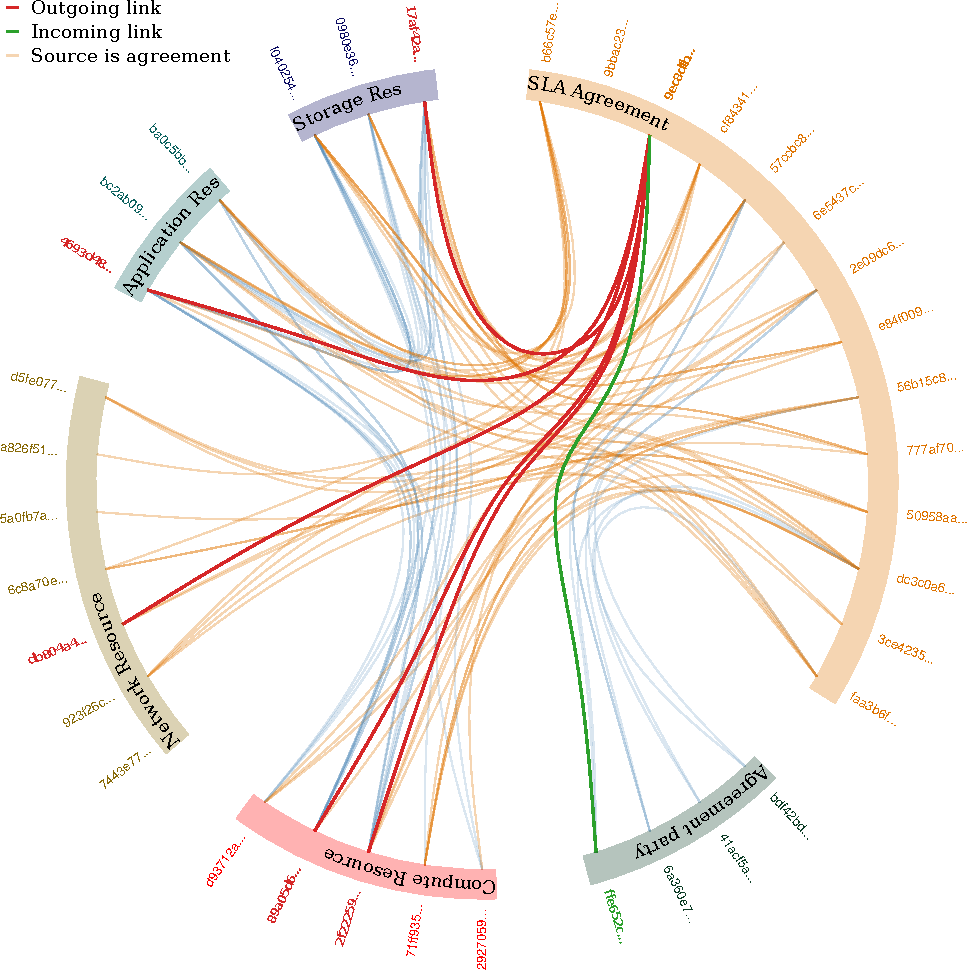
\includegraphics[width=0.9\textwidth]{images/occi.pdf}
		\caption{\emph{OCCI} verknüpft Dienstgüte-Vereinbarungen mit verteilten Anwendungen, Stakeholdern und Cloud-Ressourcen. Die Zuordnung erfolgt Service-bezogen. In der Abbildung ist eine Vereinbarung markiert: Sie wird von einem Anwender beantragt (grüne Linie) und wirkt anschließend auf Ressourcen und darauf aufbauenden Anwendungen (rote Linien). Visualisierung über \emph{OCCIViz}\protect\footnotemark.}	
		\label{fig:occi}
	\end{figure}

	\footnotetext{\url{https://github.com/IntelLabsEurope/OCCIViz}}
	
	Auch hier existiert eine experimentelle Implementierung für OpenStack\footnote{\url{https://github.com/openstack/ooi}}. Diese ist jedoch bereits als obsolet gekennzeichnet. Die SLA-Unterstützung ist über ein weiteres Projekt theoretisch verfügbar\footnote{\url{https://github.com/IntelLabsEurope/OCCI-SLAs}}.
	
	\emph{TOSCA} und \emph{OCCI} überschneiden sich nicht: Letzteres dient nicht der Modellierung providerübergreifender Infrastrukturen, sondern ausschließlich der Kommunikation mit der Plattform. Beide Standards ergänzen sich außerdem mit dem \emph{Cloud Data Management Interface (CDMI\footnote{\url{https://www.snia.org/cloud}})} für Verwaltung und Zugriff auf Netzwerkspeicher \cite{snia:2015:cdmi}. Konzeptionell wurden die Standards bereits zu einem modellbasierten Cloud-Orchestrationstool verbunden \cite{korte:2017:toscamp, carrasco:2018:toscamp}.
	%Model Driven Cloud Orchestration by Combining TOSCA and OCCI (Position Paper)
	%Fabian Korte, Johannes Martin Erbel, Jens Grabowski
	
	Um sinnvoll nutzbar zu sein, müsste der offene API-Standard von Cloud-Providern implementiert werden. Da dies nicht absehbar ist, bleibt \emph{OCCI} zumindest als interessante Grundlage für die API einer eigenen Cloud-Management-Plattform. Als pragmatischer Ersatz für den Zugriff auf Public-Cloud-Angebote, muss der Einsatz einer Multi-Cloud-Bibliothek evaluiert werden, siehe \autoref{sec:bibliotheken}.		
	
\end{description}

\noindent
Container sind nicht für jede Anwendung einsetzbar. Entsprechend müssen auch klassische virtuelle Maschinen bei einer Multi-Cloud-Migration unterstützt werden. Proprietäre Lösungen sind genauso ungeeignet wie Teillösungen auf einer einzelnen Service-Ebene.

Insgesamt ist der Support für offene Standards im Open-Source-IaaS-Projekt OpenStack am größten. Auf allen Ebenen der Service-Bereitstellung sind zumindest experimentelle Implementierungen verfügbar: \emph{cloud-init} zur Imagekonfiguration, \emph{TOSCA} zur Service-Definition und \emph{OCCI} zur Kommunikation mit der Cloud unter Berücksichtigung von SLAs. 

Einige weitere technische Herausforderungen löst ein Multi-Cloud-Broker oder eine CMP: Management von statischen und virtuellen IPs, SSL-Zertifikaten, sowie Load-Balancing. Andere Migrationshürden bleiben: Verfügbarkeit von Betriebssystemen, Frameworks und Bibliotheken, ebenso wie die Vereinbarkeit mit vorhandenen Lizenzen. Der folgende Abschnitt gibt eine Übersicht kommerzieller Cloud-Management-Plattformen sowie bisheriger Forschung zu Inter- und Multi-Cloud-Brokern mit besonderem Blick auf SLAs und Policys. 

\section{Die Limitierungen Kommerzieller CMPs}

Kommerzielle Anbieter wie \emph{RightScale} betonen den Self-Service-Charakter und potenzielle Kosteneinsparungen durch ihre Cloud-Management-Lösungen: Traditionell werden virtuelle Maschinen bei Bedarf von der internen IT bereitgestellt. Dabei entstehen auf der einen Seite Wartezeiten und auf der anderen erhöhter Arbeitsaufwand.

Eine CMP kann diese Arbeiten automatisieren. Sie helfe laut \emph{Rightscale} die \emph{Schatten-IT} abzubauen -- die entsteht, wenn Mitarbeiter aufgrund langwieriger interner Prozesse zu Public-Cloud-Angeboten greifen -- mit allen negativen Folgen für Sicherheit und Vertraulichkeit. Die automatische Durchsetzung von Policys könnte sich also doppelt lohnen. Nebenbei liefert die CMP einen Preis- und Feature-Überblick der internen und öffentlichen Angebote. So hilft sie, das optimale Angebot zu finden.

Nichtsdestotrotz sollte die CMP unabhängig entwickelt und betrieben werden. Cloud-Provider-eigene Lösungen werden daher nicht betrachtet. Weniger geeignet sind auch SaaS-Angebote: Hier entsteht eine neue Abhängigkeit und \emph{Single-Point-of-Failure}. Die nachfolgende Aufzählung zeigt die aktuell verbreitetsten CMP-Lösungen mit besonderem Fokus auf Bereitstellungsmodelle, Funktionsumfang und Offenheit der Schnittstellen.

\todo{(Zusatz) Tabelle OS + Kommerziell}

%Automatisierung oder nur schöne Dashboards?

\begin{description}
	
	\item[Red Hat CloudForms\footnotemark]\footnotetext{\url{https://www.redhat.com/en/technologies/management/cloudforms/}}
	Kommerzielle Cloud-Management-Plattform, Grundlage ist das Open Source-Projekt  \emph{ManageIQ}\footnotemark\footnotetext{\url{https://manageiq.org/}}, das alle wichtigen IaaS-Provider unterstützt (AWS, Azure, GCP, OpenStack).
	
	Besonderheit: ein umfangreiches -- optional grafisches -- Policy-Management. Eigene Regeln folgen dem Schema \emph{Bedingung/Ereignis-Aktion}.
	
	Alle Schnittstellen der CMP sind proprietär. Die Orchestrierung liest jedoch vorhandene Vorlagen aus \emph{AWS CloudFormation} and \emph{OpenStack Heat}.
	%http://manageiq.org/docs/reference/latest/doc-Policies_and_Profiles_Guide/miq/
	
	\item[Rightscale CMP\footnotemark]\footnotetext{\url{https://www.rightscale.com/}}
	Proprietäres \emph{Software-as-a-Service}-Angebot, unterstützt alle wichtigen IaaS-Provider, zusätzlich Plattformdienste, Docker-Container und Hypervisoren, besonders \emph{VMware vSphere}.
	
	Infrastruktur und Dienste werden als Vorlagen in einem eigenen Katalog bereitgestellt. Dabei erlaubt Rightscale auch heterogene Anwendungen über IaaS-, CaaS- und PaaS-Grenzen hinweg.
	
	Ein Dashboard zeigt Empfehlungen zur Kostenoptimierung, allerdings ohne SLAs einzubeziehen.
	
	\item[Scalr\footnotemark]\footnotetext{\url{https://www.scalr.com/}} war ursprünglich quelloffen unter GPL verfügbar. Diese Version wurde nach kurzer Ankündigung\footnote{\url{https://groups.google.com/forum/\#!topic/scalr-discuss/khFayhYJlhA}} im September 2017 innerhalb weniger Tage eingestellt. Seit dem existiert ausschließlich eine kommerzielle Closed-Source-Variante zum Betrieb auf eigener Hardware.	
	
	Verteilte Anwendungen werden mithilfe des \emph{Farm Builders} deklarativ in einer proprietären YAML-Datei beschrieben. Die Zuteilung von Cloud-Providern und Ressourcen ist explizit. Zusätzliche Regeln sind optional, werden aber nicht für ein Cloud-Brokering genutzt. Über einen internen Katalog können so beschriebene Anwendungen veröffentlicht werden.
	
	Die Policy-Unterstützung fokussiert sich auf Zugriffsrechte, Namenskonventionen, Kostenalarme und die Erfüllung bestimmter Audit-Anforderungen. Das Interface ist service- und anwenderbezogen. Dabei entsteht eine echte Abstraktion verschiedener Cloud-Infrastrukturen. Alle Funktionen sind jedoch nur für Amazon EC2 verfügbar.
	
	\item[Cloudify\footnotemark]\footnotetext{\url{https://cloudify.co/}} implementiert den \emph{TOSCA}-Standard und ist in einer Open-Source-Version erhältlich. Mithilfe (grafischer) Werkzeuge lassen sich Cloud-In\-fra\-struk\-tur\-en und Services modellieren. Plugins erweitern Cloudify um wichtige Provider; sowohl auf IaaS- (AWS, Azure, GCP, OpenStack) als auch auf CaaS-Ebene (Kubernetes). Konfiguration wie das Start-Skript kann direkt übergeben, oder über ein Tool wie Puppet weitergeleitet werden. 
	
	Einfache Policys sind integriert, mithilfe eines rudimentären Monitorings und der Provider-Plugins werden diese umgesetzt. Der (grafische) TOSCA-Editor und echtes Cluster-Management sind allerdings nur in der proprietären Enterprise-Ausgabe enthalten.


\end{description}

Die kommerziellen Cloud-Management-Plattformen fokussieren sich auf Kostenoptimierungen und Zugriffskontrolle. Portabilität von Anwendungen und Daten spielt aber nur eine untergeordnete Rolle. Ein Brokering auf SLA-Basis findet entgegen den Werbeversprechen nicht statt. Inwieweit Forschungsprojekte diese Lücke schließen können, prüft der nächste Abschnitt.

% https://www.embotics.com/solutions-cloud-governance
% Nur Azure und Amazon. Cloud Governance: Die richtigen Meta-Tags zu Instanzen hinzufügen. Kostenoptimierungsvorschläge, aber nur die Wahl zwischen zwei Providern.


%DivvyCloud (Commercial) 
%
%Automation Bots to schedule downtime, terminate, or re-size instances and resources so you only pay for what you use 
%
%https://divvycloud.com/product/botfactory/for-cost/ 

%
%Commercial Tools 
%
%https://www.cloudyn.com/ 
%
%close-source 
%
%only cost monitoring and optimization 
%
%Also, Cloudhealth, CloudCheckr 


\section{Bisherige Forschungsarbeiten}

Besonders interessant sind bisherige Arbeiten, die neben einer Föderation auch Hybrid- oder Multi-Cloud-Brokering unterstützen. Es sollten also keine Cloud-internen Plugins oder Agenten nötig sein.

Die folgende Übersicht geht besonders auf den Umfang der Policy- und SLA-Fähigkeiten ein: Diese sollten nicht nur während des Brokerings beachtet werden, sondern kontinuierlich zur Laufzeit. Auch die Einhaltung von Standards zu Service- und Ziel-Definitionen, sowie Kommunikation sind relevant. Unterschiede gibt es bei der Art unterstützter Anwendungen; neben Stapelverarbeitungsjobs und High-Performance-Computing sollten auch reguläre, interaktive Web-Anwendungen verwaltet werden können. 

Auch nicht-funktionale Anforderungen werden betrachtet: Sind die Artefakte der Projekte noch als Code verfügbar oder sogar in Open-Source-Tools und kommerziellen Produkten aufgegangen?

%policy-driven service placement optimization in federated clouds

\begin{description}	
	
	
	\item[InterCloud] ist ursprünglich eine Föderation von Cloud-Ressourcen \cite{buyya:2010:intercloud}. Auf einem zentralen Marktplatz \emph{zeigen} Clouds ihre Dienste, oder \emph{kaufen} sie je nach Bedarf. Für diese aktive Teilnahme sind Cloud-interne Agenten nötig.
	
	Vorgeschlagen werden zusätzlich externe Adapter, über die einerseits Provider \emph{unfreiwillig} in die Föderation integriert werden, andererseits aber auch weitere Teilnehmer Ressourcen kaufen können. Hierüber könnten auch Anwendungsbroker die Ressourcen der Föderation nutzen.
	
	Der Ansatz fokussiert sich stark auf das preisgesteuerte Brokering, beachtet optional aber auch Geostandorte. Die Provider unterstützen eingeschränkt SLAs. Verteilt werden nur Rechenaufgaben, interaktive Anwendungen sind nicht vorgesehen.
	%	5, 37, 38 Grozev	
	
	\item[Contrail] ist eine zentral gemanagte Föderation \cite{carlini:2011:contrail}. SLAs gelten für den gesamten Cloud-Verband, nicht für einzelne Anwendungen. Das zentrale Element, der \emph{Federation-Runtime-Manager}, verteilt jedoch individuelle Nutzeranfragen und beachtet dabei Preis und Leistung.
	
%	http://contrail-project.eu/architecture

	Contrail versteht sich als PaaS und unterstützt auch \emph{Hadoop}. Ähnlich zu \emph{InterCloud} sprechen externe Adapter theoretisch weitere Provider an, die sich der Föderation nicht bewusst sind.
			
	
	\item[RESERVOIR] entwickelt eine Peer-to-Peer-Föderation mit eigenen Service-Schemata und Inter-Cloud-Protokollen \cite{rochwerger:2009:reservoir}. Ein Unterprojekt abstrahiert die Cloud-Ressourcen durch eine zusätzliche Schicht, sodass Java-Anwendungen transparent auf allen Providern ausgeführt und migriert werden können \cite{rochwerger:2011:reservoir-multi-cloud}. Ein Broker beobachtet Performance-SLAs und skaliert die Instanzen entsprechend.
%	IBM, Telefonica, SAP + Universites, EU-funded
	
	
	\item[Optimis] baut auf eine zentrale \emph{Deployment Engine (DE)} \cite{ferrer:2012:optimis}. Über interne und externe Adapter verbinden sich Cloud-Provider und senden ihre Ressourcen-Angebote. Soll eine Anwendung ausgerollt werden, wählt die DE passende Provider aus und sendet ihnen ein SLA-Template. Diese antworten mit einer Zusage, Absage oder einem Gegenvorschlag. Aus allen Antworten wählt der DE anschließend das beste Angebot. Dabei beachtet sie quantitative Größen wie den Preis, aber auch Erfahrungswerte wie Zuverlässigkeit oder die Energieeffizienz eines Providers.
	
	Die internen Adapter vertreten Föderationsmitglieder -- sie lehnen eine Anfrage des DE ab, wenn sie für den Cloud-Provider finanziell unattraktiv ist. Eine weitere Komponente, der \emph{Service-Optimizer}, beobachtet alle Anwendungen auf SLA-Verletzungen. Wie genau SLAs spezifiziert werden können, ist nicht deutlich. Auch der Matching-Algorithmus ist nicht öffentlich. Geostandorte werden nicht beachtet. Externe Adapter sind rein konzeptionell und nicht implementiert.
	
	Die Arbeit geht auch auf die Bereitstellung von Laufzeitumgebungen und Provider-spezifischen Images ein: Er schlägt eine Erweiterung des \emph{Open Virtualization Formats (OVF)} vor. Zusätzliche Metadaten beschreiben die nötige Cloud-Konfiguration.
	
	
	\item[Bernsetein InterCloud Blueprint] Eine weltweite Föderation der Cloud-Ressourcen \cite{bernstein:2011:intercloud}. Interessant ist der dezentrale Ansatz des Brokerings. Nur in dieser Arbeit wird der Broker als \emph{Single-Point-of-Failure} erkannt: Deshalb soll er zwangsläufig repliziert und in allen Regionen mindestens einmal verfügbar sein. Der Ansatz folgt also den Grundlagen des Internets und entwickelt eigene Inter-Cloud-Protokolle auf Basis von XMPP und RDF.
	
	
	\item[STRATOS] ist eine Cloud-Management-Plattform mit integriertem Multi-Cloud-Broker \cite{pawluk:2012:stratos}. Anwendungen werden über das eigenentwickelte, XML-basierte \emph{Topology Descriptor File (TDF)} beschrieben. Es enthält die Service-Architektur und zusätzlich Policys und SLOs. Für den Zugriff auf externe Clouds existiert ein \emph{Translation-Layer}, der eine einheitliche API bereitstellt. Die Arbeit fokussiert sich auf die Bereitstellung klassischer Web-Anwendungen und Kostenoptimierung. Der mittlerweile nicht mehr weiterentwickelte \emph{Service Measurement Index (SMI)} definiert die Ziele.
%	https://www.google.de/url?sa=t&rct=j&q=&esrc=s&source=web&cd=1&ved=0ahUKEwju27vHs6DZAhUCWRQKHRv7BEcQFggrMAA&url=http%3A%2F%2Fwww.mikesmit.com%2Fwp-content%2Fpapercite-data%2Fpdf%2Fcloud2012.pdf&usg=AOvVaw3e6yhHYmhWBbIxtr7MqkuX
	
	\item[Meryn] ist eines der wenigen Implementierung eines SLA-bezogenen PaaS-Systems \cite{dib:2013:meryn}. Aktuelle Plattformen begrenzen hauptsächlich den Ressourcenverbrauch der Gastanwendungen -- Meryn schlägt zusätzlich eine Kostenoptimierung für Provider vor.
	
	Cloud-interne \emph{Cluster-Manager} bieten in einem Wettbewerb um Ausführungsaufträge. Die Arbeit fokussiert sich auf Stapelverarbeitung mit Hadoop und anderen Framworks. Dabei entwickeln die Autoren für jedes Framework eine eigene VM, die jeweils einmal pro Cluster ausgeführt wird. Vorgestellt wird außerdem ein \emph{Cloud-Bursting-Ansatz}, bei dem zusätzliche Ressourcen in Public Clouds angemietet werden.
	
	
	\item[SeaClouds] ist ein EU-finanziertes PaaS-Management-Projekt mit großem Umfang \cite{seaclouds:2015:architecture}. Vorgeschlagen wir ein Referenzmodell aus \emph{Planner}, \emph{Deployer}, \emph{SLA-Service} und \emph{Monitor}. Hierüber lassen sich verteilte Anwendungen modellieren, auf verschiedenen Providern bereitstellen und SLA-bezogen verwalten.
	
	Besonderheit ist die Unterstützung von offenen Standards wie der \emph{Cloud Application Management for Platforms (CAMP)} für APIs und TOSCA zur Service-Modellierung. Angebote der Cloud-Provider werden kontinuierlich überwacht und als \emph{TOSCA}-Graph abgebildet. SLAs nutzen allerdings nicht \emph{TOSCA}, sondern \emph{WS-Agreements}.
%	http://wsag4j.sourceforge.net/site/wsag/wsag-language.html
		
	Erwähnt wird eine Provider-unabhängige Lösung, konkret umgesetzt ist dies jedoch nur für die Open-Source-PaaS-Projekte \emph{OpenShift} und \emph{CloudFoundry}.
	
	\item[TOSCAMP] oder \emph{End-to-End Orchestration of
	Multi-Cloud Applications}, kombiniert in einem Prototyp die Standards \emph{TOSCA} und \emph{CAMP} \cite{korte:2017:toscamp}. Eine verteilte Anwendung wird abstrakt als \emph{TOSCA}-Template inklusive einfacher Policys beschrieben. Anschließend wandelt \emph{TOSCAMP} diese Beschreibung in einen \emph{CAMP}-Plan zur Multi-Cloud-Installation.

	Im Gegensatz zu anderen Cloud-Management-Plattformen erstellt \emph{TOSCAMP} keinen internen Graphen einer Anwendung -- stattdessen erweitert die Arbeit \emph{CAMP} um Policys und bildet alle Installationen in einer YAML-Datei ab. Einen ähnlichen Ansatz verfolgt das Projekt \emph{brooklyn-tosca\footnote{\url{https://github.com/cloudsoft/brooklyn-tosca}}}.
	
%	\item[An SLA-based Broker for Cloud Infrastructures] Nicht nur Private Clouds sondern auch Personal Devices 
%	
%	Modulare Architektur 
%	
%	wechselnde und unzuverlässige Provider
%	
%	Fokus auf Föderation. Aber: Idee der forced integration of commercial cloud providers 
	
\end{description}

%Mist.io Open source 
%Build on libcloud and cloudify
%Can monitor costs (commercial)
%No automatic scheduling 

\noindent
Im Gegensatz zu den kommerziellen Projekten liegt der Fokus vieler Forschungsarbeiten auf Cloud-Föderationen und SLA-basiertem Brokering. Einige unterstützen über Adapter konzeptionell mehrere Bereitstellungsmodelle; je nachdem, ob dem Cloud-Provider die Mitgliedschaft in einer Föderation bewusst ist. Interne Adapter sprechen mit zusätzlichen, Cloud-internen Erweiterungen. Externe Adapter nutzen die öffentlichen APIs von Drittanbieter-Clouds. Hier entsteht zwar Mehraufwand, dieser könnte in weiteren Entwicklungen jedoch von einer Multi-Cloud-Bibliothek abgefangen werden.

Negativ fällt auf, dass die Artefakte der meisten (EU-)Forschungsprojekte
nicht mehr verfügbar sind. Auch Matching-Algorithmen sind teilweise nicht veröffentlicht. Die Ergebnisse lassen sich so nicht mehr nachvollziehen. Ohnehin basieren sie oft auf veralteten Technologien: Formate wie \emph{OVF} werden in modernen IaaS-Plattformen nicht mehr unterstützt. Demgegenüber spielen Container oder Serverless-Computing in früheren Projekten keine Rolle.

Wie bereits beschrieben, existieren eine Vielzahl von offenen Cloud-Standards \cite{bmwi:2012:cloud-standards}; von Service-Definition, über SLAs, bis zur standardisierten Kommunikation mit der Managementplattform -- aber weder in der Forschung noch im kommerziellen Umfeld werden diese Standards aufgegriffen. Stattdessen erfindet man sie immer wieder neu. Besonders deutlich wird dies in einer Forschungsübersicht der Europäischen Kommission \cite{blasi:2013:eu-projects-overview}. Das eigentliche Problem der Portabilität im Cloud-Umfeld lässt sich so nicht lösen.

Insgesamt bleibt vor allem die unterschiedliche Ausrichtung von Forschungsprojekten und kommerziellen Anbietern: Forschungsprojekte fokussieren sich auf Föderationen. Dies entspricht auch dem vorherrschenden Cloud-Typ innerhalb der verantwortlichen Organisationen. SLAs werden ausschließlich von diesen ausgewertet und teilweise umgesetzt. Kommerzielle Projekte sind dagegen meist externe Broker, stellen Preisunterschiede und Kosten dar. Statt SLAs beachten sie nur einfache Policys.

Das folgende Kapitel erstellt aus den bisherigen Überlegungen zu Anforderungen, Schemata und Forschungsergebnissen einen Vorschlag für SLA-basiertes Brokering auf Basis moderner Technologien.
